% fig_pipeline_tikz.tex
% Standalone TikZ source for the corrected HiED pipeline figure.
% Compile:  pdflatex fig_pipeline_tikz.tex   ->  fig_pipeline_tikz.pdf
% Then copy/rename to fig_pipeline.pdf in paper/drafts, paper/school, paper/jbhi.
% The three .tex files keep their existing 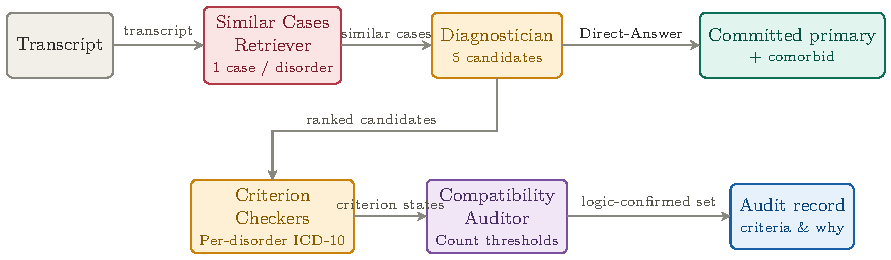
\includegraphics{fig_pipeline.pdf} unchanged.

\documentclass[border=3pt]{standalone}
\usepackage{tikz}
\usetikzlibrary{positioning, arrows.meta}
\usepackage{helvet}
\renewcommand{\familydefault}{\sfdefault}

\definecolor{procFill}{HTML}{F1EFE8}
\definecolor{procDraw}{HTML}{888780}
\definecolor{procText}{HTML}{2C2C2A}
\definecolor{decFill}{HTML}{E1F5EE}
\definecolor{decDraw}{HTML}{0F6E56}
\definecolor{decText}{HTML}{085041}
\definecolor{audFill}{HTML}{E6F1FB}
\definecolor{audDraw}{HTML}{185FA5}
\definecolor{audText}{HTML}{0C447C}

\begin{document}
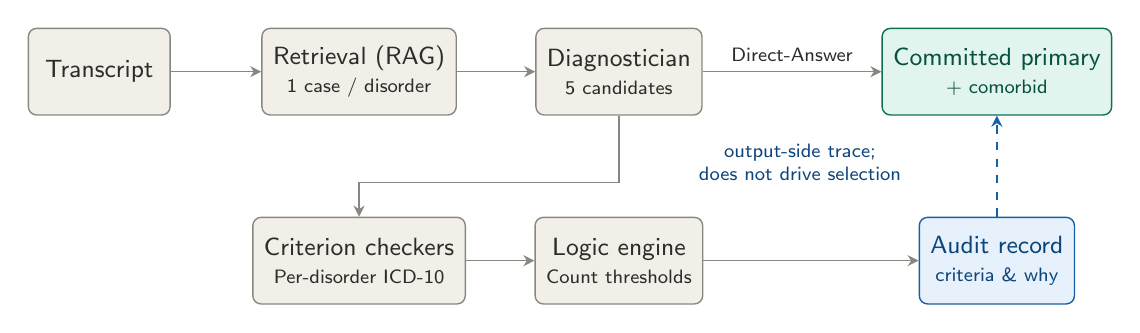
\begin{tikzpicture}[
  font=\small,
  box/.style={rectangle, rounded corners=3pt, draw, line width=0.5pt,
              align=center, inner sep=4pt, minimum height=11mm, minimum width=18mm},
  proc/.style={box, fill=procFill, draw=procDraw, text=procText},
  dec/.style={box,  fill=decFill,  draw=decDraw,  text=decText},
  aud/.style={box,  fill=audFill,  draw=audDraw,  text=audText},
  arr/.style={-{Stealth[length=4pt,width=4pt]}, line width=0.5pt, draw=procDraw},
  darr/.style={-{Stealth[length=4pt,width=4pt]}, line width=0.6pt, draw=audDraw, dashed},
]

% ---- Row 1: selection path ----
\node[proc] (tx)  at (0,0)     {Transcript};
\node[proc] (rag) at (3.3,0)   {Retrieval (RAG)\\[-1pt]{\scriptsize 1 case / disorder}};
\node[proc] (dx)  at (6.6,0)   {Diagnostician\\[-1pt]{\scriptsize 5 candidates}};
\node[dec]  (pri) at (11.4,0)  {Committed primary\\[-1pt]{\scriptsize + comorbid}};

% ---- Row 2: audit branch ----
\node[proc] (chk)   at (3.3,-2.4)  {Criterion checkers\\[-1pt]{\scriptsize Per-disorder ICD-10}};
\node[proc] (logic) at (6.6,-2.4)  {Logic engine\\[-1pt]{\scriptsize Count thresholds}};
\node[aud]  (audit) at (11.4,-2.4) {Audit record\\[-1pt]{\scriptsize criteria \& why}};

% ---- Selection-path arrows ----
\draw[arr] (tx)  -- (rag);
\draw[arr] (rag) -- (dx);
\draw[arr] (dx)  -- node[above, font=\scriptsize, text=procText] {Direct-Answer} (pri);

% ---- Branch: candidates feed the checkers ----
\draw[arr] (dx.south) -- ++(0,-0.85) -| (chk.north);

% ---- Audit-branch arrows ----
\draw[arr] (chk)   -- (logic);
\draw[arr] (logic) -- (audit);

% ---- Output-side annotation ----
\draw[darr] (audit.north) -- (pri.south);
\node[font=\scriptsize, text=audText, align=center] at (8.9,-1.15)
     {output-side trace;\\does not drive selection};

\end{tikzpicture}
\end{document}
